\section{Aufgaben}

\subsection{26.04}
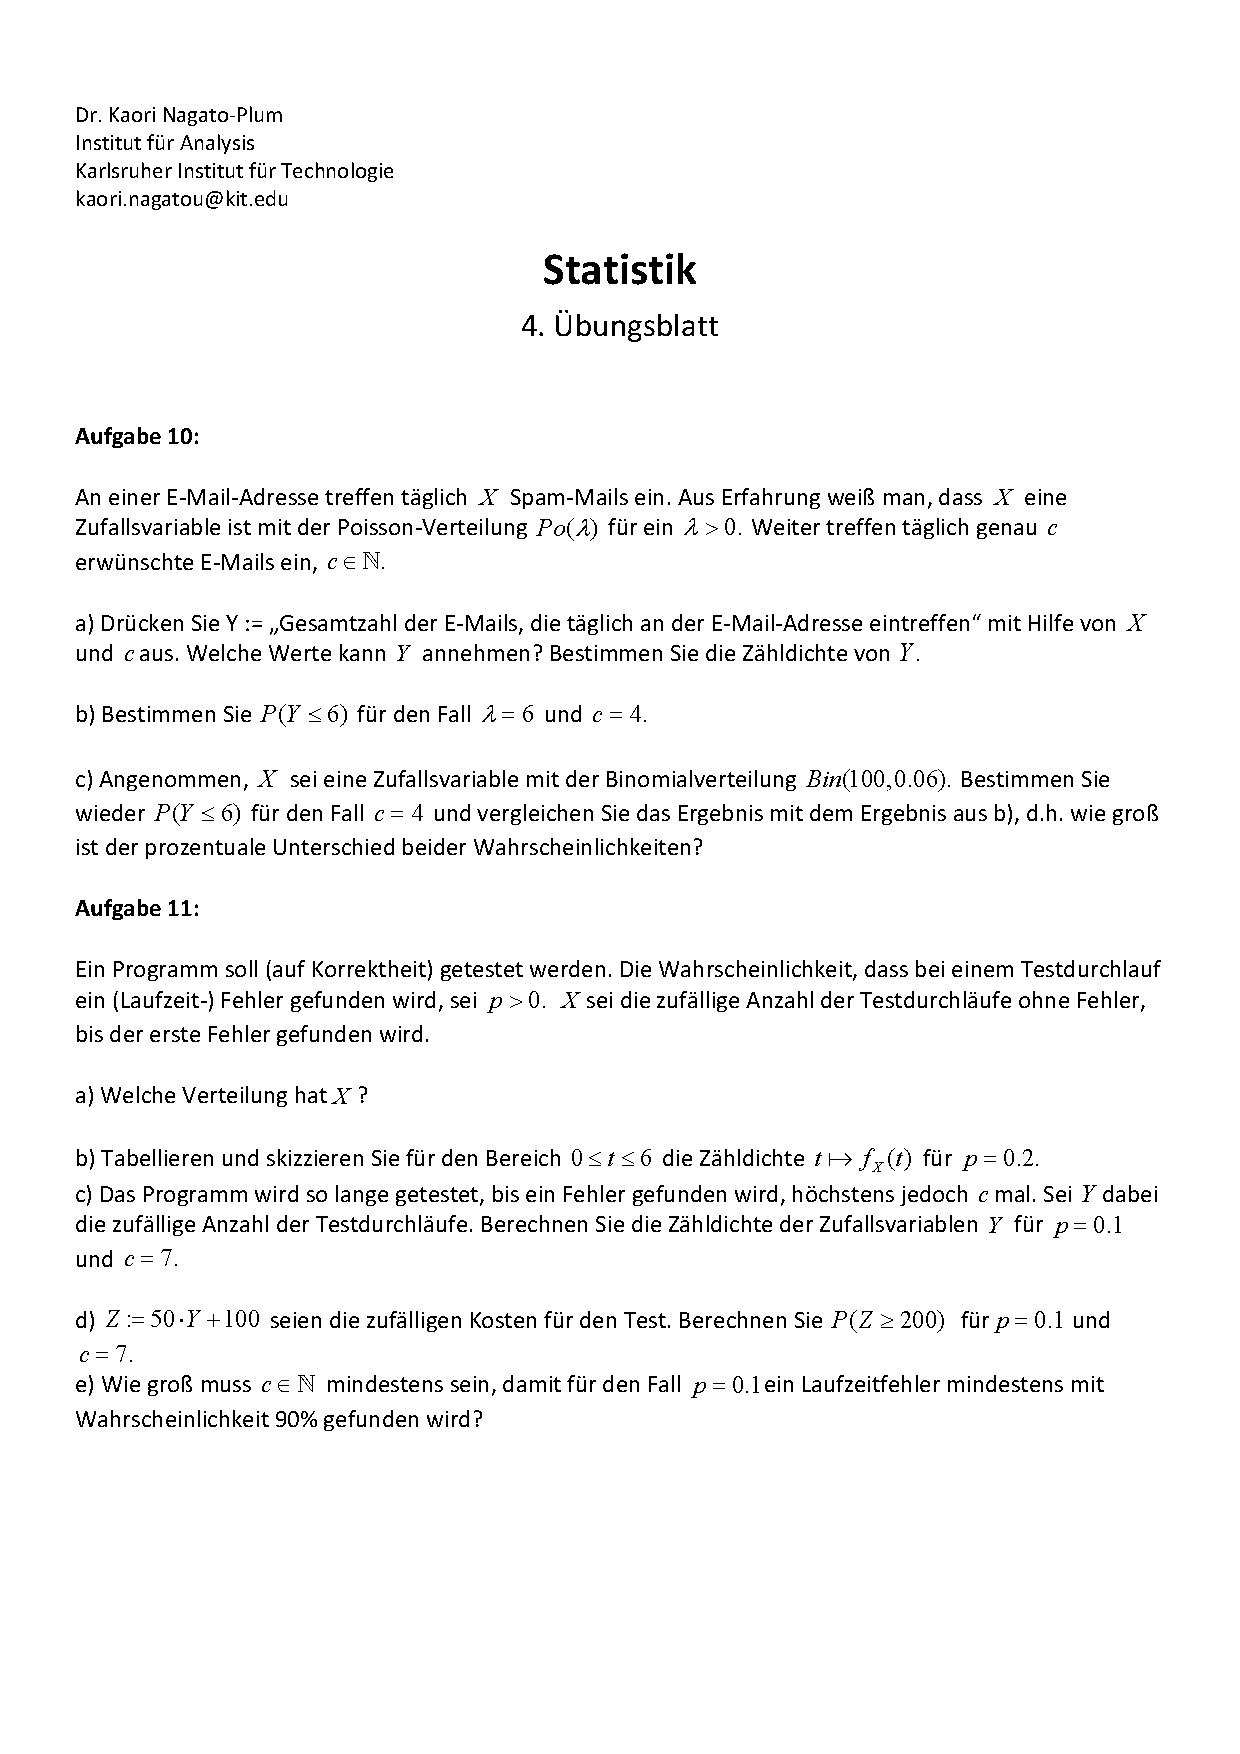
\includegraphics[scale=0.75,page=1]{input/grahix/Aufgabenblatt4.pdf}

Nur AUfgabe 10 war klausurrelevant.

Aufgabe 10 a.\\

Die Zähldichte für $Y$ ist folgend definiert $Y = X+c$. Da $X$ die Werte 0,1... annehmen kann, nimmt $Y$ die Werte c,c+1,c+2,... an. \\

\[f_Y(k)=P(Y=k)=P(X+c=k)=P(X=k-c)\]
\[f_X(k-c)=\begin{cases}e^{\lambda}*\frac{\lambda^{k-c}}{(k-c)!},k\geq c\\
0\end{cases}\]

Aufgabe 10 b.\\

Wegen $Y\geq c =4$ gilt $P(Y\leq 6)=P(Y=4)+P(Y=5)+P(Y=6)$



Die verteilung ist 








\subsection{03.05}

Aufgabe 15 a.\\

Bestimme die Dichtefunktion:

\[F(x)=1-e^{-kx}\]
\[f(x)=k*e^{-kx}\]

Für einen bestimmten Bauteil ist k = 1. Wie groß ist dann die Wahrscheinlichkeit, dass die Lebensdauer 
b. höchstens 1 Jahr \\

\[\Longrightarrow P(L\leq1)=F_1(1)-F_1(0)=1-e^{-1*1}-0=0.6321\]


c. zwischen 1 und 2 Jahren \\

\[ \Longrightarrow P(1 \leq L \leq 2) = F_1(2)-F_1(1) = (1-e^{-1*2}) -0.6321 = 0.2325\]


d. größer als 2 Jahre ist?\\

\[ \Longrightarrow P(L\geq 2) = 1-(F_1(2)-F_1(0))=0.13533\]

\subsection{10.05}

Aufgabe 16 a.\\

\[Y = N (0,16)\]

\[X=\tau + Y\]
\[ Y \sim  N(0,4^2)\]
\[\Longrightarrow X = \tau + Y = (\tau/a) + (1/b) * Y\]
\[\sim  N(\overbrace{a+b\mu}^{=\tau} ,\overbrace{b^2*\sigma ^2}^{= 4^2})\]
\[X \sim N(\tau, 4^2)\]
\[\Longrightarrow P(X\leq 100)\]

b.\\

\[\Phi (\frac{\overbrace{t}^{100}-\overbrace{\mu}^\tau}{\sigma})\]
\[\mu_0 = 1-(P\leq 100) = p_0=\Phi (\frac{\overbrace{t}^{100}-\overbrace{\mu}^{100}}{\sigma})=\Phi(0)=0.5 \]
\[\mu_1 = 1-(P\leq 102) = p_1=\Phi (\frac{\overbrace{t}^{100}-\overbrace{\mu}^{102}}{\sigma})=\Phi(-0.5)= 0.6915\]

c.\\

Jeder der vier Fühler hat die Wahrscheinlichkeit von 50$\%$ anzuschlagen bei der Temperatur 100 Grad es braucht zwei damit der Ventiator angeht.
\[N\sim Bin(4,p)=P(N=k)=\binom{4}{k}*0.5^k*0.5^{4-k}\]
\[P(N=2)+P(N=3)+P(N=4)\]
Die Wahrscheinlichkeit das der Ventilator angeht liegt bei 43.75 Prozent.\\

d.\\

\[p=0.6915\]\[ P(N\geq 1)\]

Aufgabe 17\\
a.\\
\[\mu =2 \vert \sigma =0.5 \vert P(X\leq 3)\]
\[P(N>3) = 1-(X\leq 3)= 1-\Phi _{2,0.5^2}(3)=1-\Phi (\frac{3-2}{0.5} )=\Phi (2)=1-0.97=0.03\]

\subsection{24.05}
Aufgabe 18 ist ein gute Übung für bedingte wahrscheinlichkeit.\\
\textbf{Aufgaben 20a}\\
Als Beispiel für bedingte wahrscheinlichkeit nutzen

Auf einem Mail-Server sind 96\% der ankommenden Mails Spam.\\
a.$)$Die Wahrscheinlichkeit liegt bei 90\% das eine Mail als Spam erkannt wird(d.h. mit 10\% das der Spam durch geht). Die Wahrscheinlichkeit das ein echte Mail als Spam erkannt wird liegt bei 2\%. Welcher Anteil der Mails, sind im langfristigen Mittel Spam-Mails?
\begin{align*}
    S&:= \textrm{der eingehenden Mails sind Spam} &\overline{S}&:= \textrm{nicht Spam}\\
    P&(S)=0.96 &P(\overline{S})&=0.04\\
    P&(S\cap L)= 0.96\cdot 0.90=0.864  &P(S\cap\overline{L})&=0.96\cdot0.10 = 0.096\\
    P&(\overline{S}\cap L)= 0.04\cdot 0.02 = 0.0008 &P(\overline{S}\cap\overline{L})&=0.04\cdot0.98 = 0.0392
\end{align*}
Es kommen 13.52\% der einkommenden Mails durch
\begin{align*}
    P(\overline{L})&= 0.1352\\
    P(S\cap\overline{L})&= 0.096\\
    P(S|\overline{L})&= \frac{P(S\cap \overline{L})}{P(\overline{L})} = \frac{0.096}{0.1352}\approx  0.71
\end{align*}


\subsection{Probeklausur}


